\subsection{実務上の考慮}

\subsubsection{要求プロセスの反復性}

現実の要求活動は、一回で終わらない。最初は広く浅く要求を集め、次に重要な部分を深く分析し、その後また不足が見つかって追加で獲得することが多い。要求は幅と深さの両方を持つため、反復的に進めるのが自然である。

ウォーターフォール型では、要求フェーズで多くの要求を先に固める。反復型やアジャイル型では、初期に高レベル要求を押さえ、その後、開発する順に詳細化する。重要なのは、ライフサイクルの名前ではなく、対象ソフトウェアの性質に合う要求活動を選ぶことである。

\subsubsection{要求の優先順位付け}

\term{要求の優先順位付け}{Requirements Prioritization}は、限られた費用と時間の中で、価値の高い要求から扱うために必要である。優先度は、価値だけでなく、未実現だった場合の不満、実装費用、保守費用、技術リスク、利用されないリスクなどを考慮して決める。

\MiniBox{Kanoモデルの考え方}{ある機能があると満足度が上がる場合と、ないと強い不満が出る場合は異なる。たとえばメールソフトでは、迷惑メールフィルタはあると嬉しい機能かもしれないが、添付ファイルを扱えないと利用者は強く不満を持つ。優先度は満足と不満の両方から考える。}

優先度の表し方には、「必須」「望ましい」「あればよい」のような段階、1から10の数値、優先順位リストなどがある。実務では、細かな数値差よりも、同程度の優先度を持つ要求群を見つけることが重要である。

\subsubsection{要求の追跡可能性}

追跡可能性とは、要求がどこから来て、どの設計、コード、テスト、文書につながるかをたどれることです。これは二つの目的で役立つ。

第一に、成果物間の整合性確認である。ある要求に対応する設計要素がなければ、その要求は満たされていない可能性がある。逆に、ある設計要素に対応する要求がなければ、その設計要素は不要か、要求が不足している可能性がある。

第二に、変更の影響分析である。ある要求が変わったとき、関連するソフトウェア要求、設計要素、コード、テストケース、利用者文書をたどることで、変更に必要な作業範囲を見積もりやすくなる。

\par\smallskip
\begin{center}
\centering
\IfFileExists{assets/generated_figures/ch01/fig-ch01-11.png}{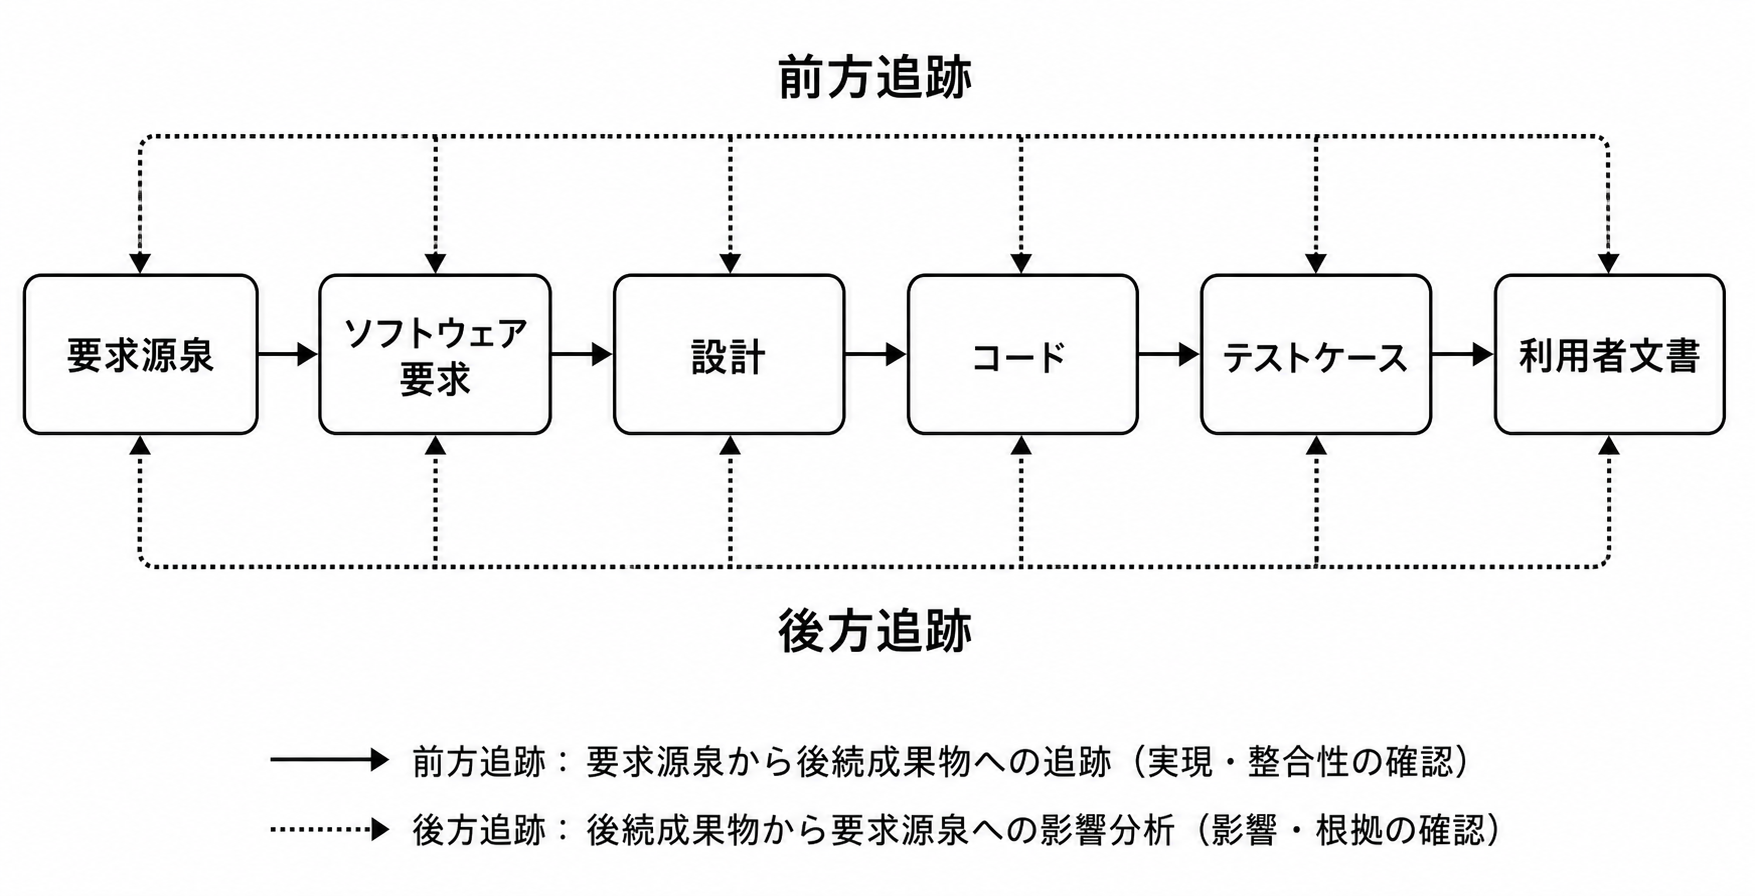
\includegraphics[width=0.96\linewidth]{assets/generated_figures/ch01/fig-ch01-11.png}}{\fbox{\parbox[c][48mm][c]{0.9\linewidth}{\centering 画像生成待ち\\要求追跡の連鎖図}}}
\par\smallskip
\refstepcounter{figure}\label{fig:ch01-11}図 \thefigure: 要求追跡の連鎖図
\end{center}
図 \thefigure は、要求追跡の連鎖図を視覚的に整理したものである。
\par\smallskip

\subsubsection{要求の安定性と変動性}

\term{要求の安定性}{Requirements Stability}とは、要求が変わりにくい度合いである。\term{変動性}{Variability}とは、要求が変わりやすい度合いである。

銀行アプリケーションで「口座に利息を計算して付与する」は比較的安定した要求である。一方、税制に基づく特定口座の扱いは、法改正で変わる可能性がある。変わりやすい要求を早く見つけると、変更に強い設計を選びやすくなる。

\subsubsection{要求の測定}

要求を測定する理由は、規模、費用、進捗、品質を管理するためである。\term{機能規模測定}{Functional Size Measurement}は、機能要求の大きさを測る技法である。アジャイル開発で使われるストーリーポイントも、要求の大きさを表す測度として使われることがある。

要求品質の指標は、曖昧さ、テスト可能性、重複、矛盾、欠落、変更頻度などから作れる。これらを測ることで、要求プロセスの弱点を改善しやすくなる。

\subsubsection{要求プロセスの品質と改善}

要求プロセスの品質は、ソフトウェア製品の費用、納期、顧客満足度に大きく影響する。要求プロセスを改善するには、プロセス改善モデルや品質標準との対応、測定、ベンチマーク、改善計画、実施、振り返りが必要である。

セキュリティの観点では、機密性、完全性、可用性をどのように要求へ反映し、改善するかも重要である。
